\begin{CJK}{Bg5}{bsmi}

%---------------------------------------------
%	Chapter System Architecture
%---------------------------------------------

\chapter{System Architecture}

In this chapter, I'll try to explain my design more detailed. First section is the basic idea of my authentication system, which is based on digital signature algorithm. The next section is about the flow if clinets and servers adopt this scheme. The next chapter gives two demonstrations of this scheme. One is for the furture website, and one if for the existing website. The last section gives a high-level code example to explain how to implement this system.

\section{Overview}

\begin{figure}
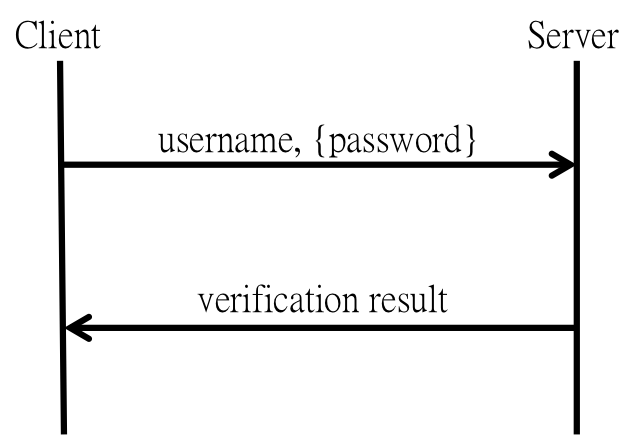
\includegraphics{picture/password-based-flow.png}
\centering
\end{figure}

\section{User Flow}

\subsubsection{Register Phase}

	1. 	User start the initialzization process on his mobile device
		i.  set PIN code
		ii. generate key pair
	2.	User send a registration request to server from browser

	3.	User send his id and public key (and other required credentials) to server.

\subsubsection{Login Phase}

	1. User send a login requesr to server

	2. Server return a nonce ({server info || randombits}) back to browser

	3. The brower pass this nonce to reader application
		i.	The reader start to scan NFC cards.
		ii.	Timeout: 30 seconds

	4. Mobile device ask user to input the correct PIN code and confirm the server information
		i.	Enable card emulation mode right after receive correct PIN code

	5. Mobile device get nonce from reader application
		i.	mobile device signed the nonce with correspond private key.
		ii.	mobile device return the signed-nonce back to reader application

	6. Reader application return signed-nonce back to server.

\subsubsection{Verification Phase}

	1. Server find the corresponding public key accordding to id.

	2. Verify the signature.

	3. Return the result.

\section{Scenario}

\subsection{Future Website}

\subsection{Existing Website}

\section{Implementation}

\end{CJK}